\documentclass[tikz,convert={outfile=\jobname.svg}]{standalone}

\usepackage{tikz, times}
\usetikzlibrary{automata,backgrounds,shapes,arrows,positioning,calc,decorations,fit,mindmap,trees,shadows,intersections,matrix}
\usepgflibrary{decorations.markings,decorations.shapes,decorations.pathreplacing,decorations.footprints,decorations.text,decorations.pathmorphing,decorations.fractals}


\tikzstyle{block} = [color=black!84,draw=black!60,fill=black!5,minimum size=2em,rounded corners=0.5mm, text centered, text width=2cm, minimum height=2cm,line width=1pt]
\tikzstyle{tnode} = [draw,color=black,minimum size=0.71cm, inner sep=0]
\tikzstyle{vblock} = [draw,color=black!55,fill=black!1,minimum size=2em,rounded corners=0.5cm, text centered, text width=2cm, minimum height=5cm,line width=1pt]
\tikzstyle{vnode} = [draw=black!55, minimum height =0.7cm,text width= 2cm, align=center]
\tikzstyle{hblock} = [draw,color=black!55,fill=black!1,minimum size=2em,rounded corners=0.2cm, text centered, text width=6cm, minimum height=0.7cm,line width=1pt]
\tikzstyle{hnode} = [draw=black!55, minimum height =0.7cm,text width= 0.7cm, align=center]
\tikzstyle{head} = [>=fast cap,->, double distance=2pt,color=black!60,line width=1.2pt]
\tikzstyle{darrow} = [>=latex',->,line width=0.6pt]



\begin{document}
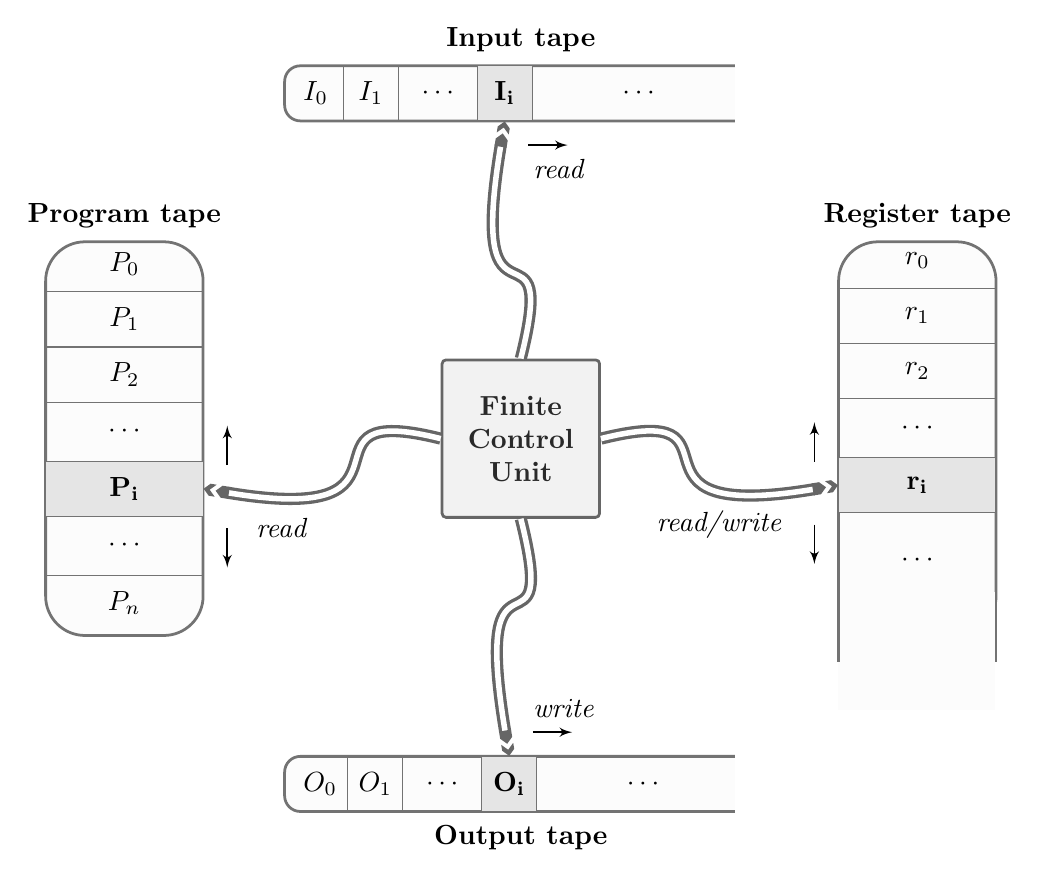
\begin{tikzpicture}[node distance=0.7cm, inner sep=0pt]% Example:
    \node[block] (ram) {\textbf{Finite Control Unit}};
    
    % program tape
    \node[vblock] (program) [left= 3cm of ram] {};
    \node[above=0.15cm] at (program.north) {\textbf{Program tape}};
      \node[below=0.15cm] (p0) at (program.north) {$P_0$};   %- (0,0.27cm)$
      \node (p1) [below of=p0,vnode] {$P_1$};
      \node (p2) [below of=p1,vnode] {$P_2$};
      \node (dots) [below of=p2, vnode, minimum height=0.75cm,yshift=-0.025cm] {$\cdots$};
      \node (pi) [vnode,below of=dots,fill=black!10,yshift=-0.025cm] {$\mathbf{P_i}$};
      \node (dotss) [below of=pi, vnode, minimum height=0.75cm,yshift=-0.025cm] {$\cdots$};
      \node (pn) [below of=dotss, vnode, draw opacity=0,yshift=-0.025cm] {$P_n$};
      
    % registers tape
    \node[vblock] (registers) [right= 3cm of ram] {};
    \node[above=0.15cm] at (registers.north) {\textbf{Register tape}};
      \node[below=0.15cm] (r0) at (registers.north) {$r_0$};
      \node (r1) [below of=r0,vnode] {$r_1$};
      \node (r2) [below of=r1,vnode] {$r_2$};
      \node (dots) [below of=r2, vnode, minimum height=0.75cm,yshift=-0.025cm] {$\cdots$};
      \node (ri) [vnode,below of=dots,fill=black!10,yshift=-0.025cm] {$\mathbf{r_i}$};
      \node (dotss) [below of=ri, vnode, draw opacity=0,yshift=-0.25cm] {$\cdots$};
      \fill[black!1] ($(dotss.west) - (0,0.4)$) rectangle +(2cm,-1.5cm);
      \draw[black!55,line width=1pt] ($(dotss.west)+(0.0071cm,-0.3)$) -- +(0,-1cm);
      \draw[black!55,line width=1pt] ($(dotss.east)-(0.0071cm,0.3)$) -- +(0,-1cm);

    
    % input tape
    \node[hblock] (input) [above= 3cm of ram] {};
    \node[above=0.15cm] at (input.north) {\textbf{Input tape}};
      \node[right=0.25cm] (i0) at (input.west) {$I_0$}; %+ (0.27cm,0)$
      \node (i1) [right of=i0,hnode] {$I_1$};
      \node (dots) [right of=i1,hnode, minimum width=1cm, xshift=0.15cm] {$\cdots$};
      \node (ii) [hnode,right of=dots,fill=black!10, xshift=0.15cm] {$\mathbf{I_i}$};
      \node (dots) [right of=ii,hnode, draw opacity=0, minimum width=2cm, xshift=1cm] {$\cdots$};
      \fill[white] ($(input.east)-(0.3cm,0.5)$) rectangle +(1cm,1cm);

    % output tape    
    \node[hblock] (output) [below= 3cm of ram] {};
    \node[below=0.15cm] at (output.south) {\textbf{Output tape}};
      \node[right=0.25cm] (o0) at (output.west) {$O_0$}; %+ (0.27cm,0)$
      \node (o1) [right of=o0,hnode] {$O_1$};
      \node (dots) [right of=o1,hnode, minimum width=1cm, xshift=0.15cm] {$\cdots$};
      \node (oi) [hnode,right of=dots,fill=black!10, xshift=0.15cm] {$\mathbf{O_i}$};
      \node (dots) [right of=oi,hnode, draw opacity=0, minimum width=2cm, xshift=1cm] {$\cdots$};
      \fill[white] ($(output.east)-(0.3cm,0.5)$) rectangle +(1cm,1cm);

    % arrows
    \draw[head] (ram.west) .. controls +(-2,0.5) and +(3,-0.5) .. (pi.east);
    \draw[head] (ram.east) .. controls +(2,0.5) and +(-3,-0.5) .. (ri.west);
    \draw[head] (ram.north) .. controls +(0.5,2) and +(-0.5,-3) .. (ii.south);
    \draw[head] (ram.south) .. controls +(0.5,-2) and +(-0.5,3) .. (oi.north);

    % head descriptions
    \draw[darrow] ($(ri.west) - (0.3,-0.3)$) -- +(0,0.5);
    \draw[darrow] ($(ri.west) - (0.3,0.5)$) -- +(0,-0.5);
    
    \draw[darrow] ($(pi.east) + (0.3,0.3)$) -- +(0,0.5);
    \draw[darrow] ($(pi.east) + (0.3,-0.5)$) -- +(0,-0.5);
    
    \draw[darrow] ($(ii.south) + (0.3,-0.3)$) -- +(0.5,0);
    \draw[darrow] ($(oi.north) + (0.3,0.3)$) -- +(0.5,0);
    
    \node at ($(ri.west) - (1.5,0.5)$) {\textit{read/write}};
    \node at ($(pi.east) + (1,-0.5)$) {\textit{read}};
    \node at ($(ii.south) + (0.7,-0.6)$) {\textit{read}};
    \node at ($(oi.north) + (0.7,0.6)$) {\textit{write}};
\end{tikzpicture}
\end{document}
